% report.tex

% change pdflatex below to xelatex if you use Chinese
% !TEX program = xelatex
\documentclass[]{beamer}

% preamble.tex

%%%%%%%%%%%%%%% Chinese %%%%%%%%%%%%%%%
%%%%% Uncomment the following lines to use Chinese
% \usepackage{xeCJK}
% \usepackage{fontspec}
%%%%%%%%%%%%%%% Chinese %%%%%%%%%%%%%%%

%%%%%%%%%%%%%%% Theme %%%%%%%%%%%%%%%
\usetheme{CambridgeUS} % try Madrid
\usecolortheme{beaver} % try beaver, dolphin, seahorse
% \usefonttheme[onlymath]{serif} % try "professionalfonts"
\usefonttheme{serif}  % standard font (same with that in ``standalone'')
% \setCJKmainfont{Microsoft YaHei} % try SimSun
% \setmainfont{Gill Sans}
% \setsansfont{Gill Sans}

\usepackage[export]{adjustbox}

\setbeamersize{text margin left = 2em, text margin right = 1em}
\setbeamercolor{footnote mark}{fg = teal}
\setbeamertemplate{itemize items}[default]
\setbeamertemplate{enumerate items}[default]

\renewcommand*{\thefootnote}{\alph{footnote}}

\usepackage{makecell}
\usepackage{tabularx}
\usepackage{booktabs}

%%%%%%%%%%%%%%% Theme %%%%%%%%%%%%%%%

\usepackage{graphicx, subcaption}

\usepackage{amssymb, pifont}
\newcommand{\cmark}{\ding{51}}
\newcommand{\xmark}{\ding{55}}

%%%%%%%%%%%%%%% Algorithms %%%%%%%%%%%%%%%
\usepackage{algorithm}
\usepackage[noend]{algpseudocode}
% for two-column algorithms
% see https://tex.stackexchange.com/a/159431.
\usepackage{varwidth}

\newcommand{\code}[2]{#1:#2}
\newcommand{\hStatex}[0]{\vspace{4pt}}
\renewcommand\algorithmicthen{}
\renewcommand\algorithmicdo{}

\algblockdefx[upon]{When}{EndWhen}%
  [3][Unknown]{\textbf{when for every} #3 \textbf{received a quorum of} #1(#2)}%
  {\textbf{end}}

\algblockdefx[upon]{WhenReceive}{EndWhenReceive}%
  [1][Unknown]{\textbf{when received} #1}%
  {\textbf{end}}

\algblockdefx[upon]{Upon}{EndUpon}%
  [1][Unknown]{\textbf{upon} #1}%
  {\textbf{end upon}}

% Remove the end blank line when using noend in conjunction with custom blocks
% See https://tex.stackexchange.com/a/172065
\makeatletter
\ifthenelse{\equal{\ALG@noend}{t}}%
  {\algtext*{EndWhen}}
  {}%
\makeatother

\makeatletter
\ifthenelse{\equal{\ALG@noend}{t}}%
  {\algtext*{EndWhenReceive}}
  {}%
\makeatother

\makeatletter
\ifthenelse{\equal{\ALG@noend}{t}}%
  {\algtext*{EndUpon}}
  {}%
\makeatother
%%%%%%%%%%%%%%% Algorithms %%%%%%%%%%%%%%%

%%%%%%%%%%%%%%% Theorems %%%%%%%%%%%%%%%
% theorems (global numbering)
\theoremstyle{definition}
\newtheorem{property}[theorem]{Property}
\newtheorem{assumption}{\textsc{Assumption}}
%%%%%%%%%%%%%%% Theorems %%%%%%%%%%%%%%%

\usepackage{caption}
\DeclareCaptionLabelSeparator{none}{}
\captionsetup{labelsep = none}

\makeatletter
\let\@@magyar@captionfix\relax
\makeatother

%%%%%%%%%%%%%%% Tables %%%%%%%%%%%%%%%
\usepackage{multirow}
\newcommand{\incell}[2]{\begin{tabular}[c]{@{}c@{}}#1\\[3pt] #2\end{tabular}}
%%%%%%%%%%%%%%% Tables %%%%%%%%%%%%%%%

%%%%%%%%%%%%%%% Figures %%%%%%%%%%%%%%%
% for fig without caption: #1: width/size; #2: fig file
\newcommand{\fig}[2]{
  \begin{figure}[htp]
    \centering
    \includegraphics[#1]{#2}
  \end{figure}
}

% for fig with caption: #1: width/size; #2: fig file; #3: fig caption
\newcommand{\figcap}[3]{
  \begin{figure}[htp]
    \centering
    \includegraphics[#1]{#2}
    \caption{#3}
  \end{figure}
}

\newcommand{\figdouble}[6]{
  \begin{figure}[h]
    \centering
    \begin{subfigure}[c]{#1\textwidth}
        \centering
        \includegraphics[width = #2\textwidth]{#3}
    \end{subfigure}
    \hfill
    \begin{subfigure}[c]{#4\textwidth}
        \centering
        \includegraphics[width = #5\textwidth]{#6}
    \end{subfigure}
  \end{figure}
}

%%%%% For Chinese %%%%%
% \renewcommand\figurename{图:\;}
% \renewcommand\tablename{表:\;}
%%%%% For Chinese %%%%%
%%%%%%%%%%%%%%% Figures %%%%%%%%%%%%%%%

%%%%%%%%%%%%%%% TiKZ %%%%%%%%%%%%%%%
\usepackage[linewidth = 1pt, framemethod = TikZ]{mdframed}
\mdfsetup{frametitlealignment=\center}

\usepackage{tikz}
\usetikzlibrary{calc, trees, positioning, arrows, arrows.meta,
  chains, shapes.geometric, decorations.pathreplacing,
  decorations.pathmorphing, shapes, matrix, shapes.symbols, fit}
\tikzset{onslide/.code args={<#1>#2}{%
  \only<#1>{\pgfkeysalso{#2}} % \pgfkeysalso doesn't change the path
}}
\tikzset{temporal/.code args={<#1>#2#3#4}{%
  \temporal<#1>{\pgfkeysalso{#2}}{\pgfkeysalso{#3}}{\pgfkeysalso{#4}} % \pgfkeysalso doesn't change the path
}}
%%%%%%%%%%%%%%% TiKZ %%%%%%%%%%%%%%%

%%%%%%%%%%%%%%% Citation %%%%%%%%%%%%%%%
% try "backend = bibtex", "backend = biber"
\usepackage[natbib = true, backend = biber, style = authoryear, maxbibnames = 99]{biblatex}
\setbeamertemplate{bibliography item}[article]
\renewcommand*{\bibfont}{\footnotesize}
% \addbibresource{xxx.bib}

\newcommand{\ncite}[1]{\violet{\footnotesize [\cite{#1}]}}
%%%%%%%%%%%%%%% Citation %%%%%%%%%%%%%%%

%%%%%%%%%%%%%%% Colors %%%%%%%%%%%%%%%
\usepackage{xcolor}

\definecolor{DarkRed}{rgb}{0.55, 0.0, 0.0}

\newcommand{\red}[1]{\textcolor{red}{#1}}
\newcommand{\green}[1]{\textcolor{green}{#1}}
\newcommand{\blue}[1]{\textcolor{blue}{#1}}
\newcommand{\purple}[1]{\textcolor{purple}{#1}}
\newcommand{\cyan}[1]{\textcolor{cyan}{#1}}
\newcommand{\violet}[1]{\textcolor{violet}{#1}}
\newcommand{\lgray}[1]{\textcolor{lightgray}{#1}}
\newcommand{\teal}[1]{\textcolor{teal}{#1}}
\newcommand{\brown}[1]{\textcolor{brown}{#1}}
\newcommand{\orange}[1]{\textcolor{orange}{#1}}

\newcommand{\hl}[2]{\fcolorbox{#1}{#1!60}{#2}}
%%%%%%%%%%%%%%% Colors %%%%%%%%%%%%%%%

%%%%%%%%%%%%%% for appendix %%%%%%%%%%%%%%%%
% http://www-ljk.imag.fr/membres/Jerome.Lelong/latex/appendixnumberbeamer.sty
% Reference: http://tex.stackexchange.com/questions/2541/beamer-frame-numbering-in-appendix
\usepackage{appendixnumberbeamer}
% Add total frame count to slides, optional. From Stefan,
% http://www.latex-community.org/forum/viewtopic.php?f=4&t=2173
\expandafter\def\expandafter\insertshorttitle\expandafter{%
  \insertshorttitle\hfill\insertframenumber\,/\,\inserttotalframenumber}
%%%%%%%%%%%%%% for appendix %%%%%%%%%%%%%%%%

%%%%%%%%%%%%%%% thankyou %%%%%%%%%%%%%%%
\newcommand{\thankyou}{
  \begin{frame}[noframenumbering]
    \begin{center}
      \fig{width = 0.618\textwidth}{figs/thankyou}
      \vspace{0.30cm}
      Hengfeng Wei (hfwei@nju.edu.cn)
    \end{center}
  \end{frame}
}
%%%%%%%%%%%%%%% thankyou %%%%%%%%%%%%%%%
% newcommands.tex

\newcommand{\file}[1]{\textsl{file: #1}}

%%%%%%%%%%%%%%% Maths %%%%%%%%%%%%%%%
\newcommand{\N}{\mathbb{N}}
\newcommand{\Z}{\mathbb{Z}}
\newcommand{\R}{\mathbb{R}}
\newcommand{\set}[1]{\{#1\}}
\newcommand{\ps}{\mathcal{P}} % for powerset
\newcommand{\emptyseq}{\emptyset} % or using <>?
\newcommand{\tuple}[1]{\langle#1\rangle} % or using (#1)?

\DeclareMathOperator*{\argmin}{argmin} % thin space, limits underneath in displays
\DeclareMathOperator*{\argmax}{argmax} % thin space, limits underneath in displays
\newcommand{\dom}{\ensuremath{\mathsf{dom}}}
\newcommand{\range}{\ensuremath{\mathsf{range}}}
\newcommand{\domain}{\textsc{domain}}
%%%%%%%%%%%%%%% Maths %%%%%%%%%%%%%%%
%%%%%%%%%%%%%%%%%%%%%%%%%%%%%%%%%%%%%%%%%%%%%%%%%%%%%%%%%%%%%%%%%%%%%%%%%%%%%%%%
\title[事务一致性验证]{数据库事务一致性高效验证技术研究}
\subtitle{}

\author[魏恒峰]{魏恒峰}
\titlegraphic{
  
\includegraphics[height = 1.5cm]{figs/nju-logo-purple}~
  
\includegraphics[height = 1.5cm]{figs/software-logo}}
\institute{hfwei@nju.edu.cn}
\date{2023 年 10 月 18 日}
%%%%%%%%%%%%%%%%%%%%
\begin{document}
\maketitle
%%%%%%%%%%%%%%%%%%%%
% overview.tex

%%%%%%%%%%%%%%%%%%%%
\begin{frame}{}
	\begin{center}
		数据库产业是我国信创产业链中的重要组成部分。

		\vspace{0.20cm}
		\fig{width = 0.95\textwidth}{figs/xinchuang-db}
	\end{center}
\end{frame}
%%%%%%%%%%%%%%%%%%%%

%%%%%%%%%%%%%%%%%%%%
\begin{frame}{}
	\begin{center}
		事务是数据库系统中的核心概念,是支撑在线交易业务的关键技术。

		\vspace{0.30cm}
		\fig{width = 0.50\textwidth}{figs/db-transactions}
	\end{center}
\end{frame}
%%%%%%%%%%%%%%%%%%%%

%%%%%%%%%%%%%%%%%%%%
\begin{frame}{}
	\begin{center}
		``隔离性''限定了事务之间的相互影响, 避免上层业务产生数据异常。

		\vspace{0.20cm}
		\fig{width = 0.50\textwidth}{figs/acid}
	\end{center}
\end{frame}
%%%%%%%%%%%%%%%%%%%%

%%%%%%%%%%%%%%%%%%%%
\begin{frame}{}
	\begin{center}
		事务一致性模型 (隔离性) 是数据库系统与上层业务之间的一种契约。

		\vspace{0.20cm}
		\fig{width = 0.60\textwidth}{figs/layers}
	\end{center}
\end{frame}
%%%%%%%%%%%%%%%%%%%%

%%%%%%%%%%%%%%%%%%%%
\begin{frame}{}
	\begin{center}
		数据库系统与客户程序的正确性是至关重要的。

		\fig{width = 0.60\textwidth}{figs/problems}

		三个事务一致性验证问题之间的递进关系
	\end{center}
\end{frame}
%%%%%%%%%%%%%%%%%%%%

%%%%%%%%%%%%%%%%%%%%
\begin{frame}{}
	\begin{center}
		三个验证问题的复杂度都很高, 某些情况下甚至是不可判定的。

		\vspace{0.30cm}
		\fig{width = 0.60\textwidth}{figs/solver-blackbox}
		\vspace{0.30cm}

		大多数解决方案都借助于高效的 SAT/SMT 求解器。
	\end{center}
\end{frame}
%%%%%%%%%%%%%%%%%%%%
% intro.tex

%%%%%%%%%%%%%%%%%%%%
\begin{frame}{}
	\fig{width = 0.70\textwidth}{figs/verifying-history}
\end{frame}
%%%%%%%%%%%%%%%%%%%%

%%%%%%%%%%%%%%%%%%%%
\begin{frame}{}
  \begin{center}
    可序列化 (Serializability): 所有事务就像按照某个全序执行一样。

    \vspace{0.30cm}
    \fig{width = 0.70\textwidth}{figs/cobra-osdi2020}
  \end{center}
\end{frame}
%%%%%%%%%%%%%%%%%%%%

%%%%%%%%%%%%%%%%%%%%
\begin{frame}{}
  \begin{center}
    为了提高性能, 很多数据库仅提供快照隔离 (Snapshot Isolation)。

    \vspace{0.30cm}
    \fig{width = 0.80\textwidth}{figs/db-si}
  \end{center}
\end{frame}
%%%%%%%%%%%%%%%%%%%%

%%%%%%%%%%%%%%%%%%%%
\begin{frame}{Snapshot Isolation (SI)}
  \begin{center}
		\resizebox{0.50\textwidth}{!}{% isolation-si-write-skew-tikz.tex

\begin{tikzpicture}[
  node distance = 1.5cm and 1.5cm,
  txn/.style = {draw, inner sep = 3pt, align = center},
  comm/.style = {arrows = {Stealth-Stealth}, ultra thick, purple}]

  \node[txn] (t-alice)
    {$x_{1} \gets \readevent(\acctone)$\\[2pt]
     $x_{2} \gets \readevent(\accttwo)$\\[2pt]
     $\text{\bf if}\; x_{1} + x_{2} > 100$ \\[2pt]
     $\quad \red{x_{1} \gets x_{1} - 100}$ \\[2pt]
     $\quad \writeevent(\acctone, x_{1})$};

  \node[txn, right = of t-alice] (t-bob)
    {$x_{1} \gets \readevent(\acctone)$\\[2pt]
     $x_{2} \gets \readevent(\accttwo)$\\[2pt]
     $\text{\bf if}\; x_{1} + x_{2} > 100$ \\[2pt]
     $\quad \red{x_{2} \gets x_{2} - 100}$ \\[2pt]
     $\quad \writeevent(\accttwo, x_{2})$};

  \node[txn, right = of t-bob] (t-carol)
    {$x_{1} \gets \readevent(\acctone)$\\[2pt]
     $x_{2} \gets \readevent(\accttwo)$};

  \node[draw, fill = yellow!50, below = of t-bob, font = \large,
    inner sep = 8pt, minimum width = 260pt] (isolation)
    {{Snapshot Isolation (SI)}};

  \node[below = of isolation,
    label = {[label distance = 5pt]above : {\large $\acctone = \accttwo = 60$}}] (db)
    {
\includegraphics[scale = 0.70]{figs/db-logo-dollar}};

  \draw[comm] (t-alice) -- (t-alice |- isolation.north);
  \draw[comm] (t-bob) -- (t-bob |- isolation.north);
  \draw[comm] (t-carol) -- (t-carol |- isolation.north);
  \draw[comm] (isolation) -- (isolation |- db.north);

  % \uncover<2->{
  \node[txn, below = 0.50cm of db, fill = green!30] (t-bob-execution)
    {$\readevent(\acctone, 60)$ \\[2pt]
     $\readevent(\accttwo, 60)$ \\[2pt]
     $\writeevent(\accttwo, -40)$};
  % }
  % \uncover<2->{
  \node[txn, left = of t-bob-execution] (t-alice-execution)
    {$\readevent(\acctone, 60)$ \\[2pt]
     $\readevent(\accttwo, 60)$ \\[2pt]
     $\writeevent(\acctone, -40)$};
  % }
  % \uncover<3->{
  \node[txn, right = of t-bob-execution, fill = red!30] (t-carol-execution)
    {$\readevent(\acctone, -40)$ \\[2pt]
     $\readevent(\accttwo, -40)$};

    \node[above = 1.50cm of t-carol-execution] (write-skew)
      {\green{\Large \textsc{Write Skew}}};
    \node[above = 0.80cm of t-carol-execution, scale = 3] (yes) {\yes};
  % }
\end{tikzpicture}}

    \vspace{0.20cm}
    \violet{Snapshot Read:} Each transaction reads data from a {\it snapshot} \\
      as of the time the transaction started.
  \end{center}
\end{frame}
%%%%%%%%%%%%%%%%%%%%

%%%%%%%%%%%%%%%%%%%%
\begin{frame}{Snapshot Isolation (SI)}
  \begin{center}
    \resizebox{0.48\textwidth}{!}{% isolation-si-lost-update-tikz.tex

\begin{tikzpicture}[
  node distance = 1.5cm and 1.5cm,
  txn/.style = {draw, inner sep = 3pt, align = center},
  comm/.style = {arrows = {Stealth-Stealth}, ultra thick, purple}]

  \node[txn] (t-alice)
    {$x \gets \readevent(\acct)$ \\[2pt]
     $x \gets x + 50$ \\[2pt]
     $\writeevent(\acct, x)$};

  \node[txn, right = of t-alice] (t-bob)
    {$x \gets \readevent(\acct)$ \\[2pt]
     $x \gets x + 25$ \\[2pt]
     $\writeevent(\acct, x)$};

  \node[txn, right = of t-bob] (t-carol)
    {$\readevent(\acct)$};

  \node[draw, fill = yellow!50, below = of t-bob, font = \large,
    inner sep = 8pt, minimum width = 260pt] (isolation)
    {{Snapshot Isolation (SI)}};

  \node[below = of isolation,
    label = {[label distance = 5pt]above : {\large $\acct = 0$}}] (db)
    {
\includegraphics[scale = 0.70]{figs/db-logo-dollar}};

  \draw[comm] (t-alice) -- (t-alice |- isolation.north);
  \draw[comm] (t-bob) -- (t-bob |- isolation.north);
  \draw[comm] (t-carol) -- (t-carol |- isolation.north);
  \draw[comm] (isolation) -- (isolation |- db.north);

  % \uncover<2->{
  \node[txn, below = 0.50cm of db] (t-bob-execution)
    {$\readevent(\acct, 0)$ \\[2pt] $\writeevent(\acct, ?)$};
  \node[below = 0.50cm of db, scale = 3.00] (t-bob-abort) {\no};
  % }
  % \uncover<6->{
  % \node[txn, below = 0.50cm of db, fill = green!50] (t-bob-retry)
  %   {$\readevent(\acct, 0)$ \\[2pt] $\writeevent(\acct, 75)$};
  % }

  % \uncover<2->{
  \node[txn, left = of t-bob-execution] (t-alice-execution)
    {$\readevent(\acct, 0)$ \\[2pt] $\writeevent(\acct, 50)$};
  % }

  % \uncover<2->{
  \node[above right = 0.20cm and 1.00cm of t-bob-execution] (lost-update)
    {\red{\large \textsc{Lost Update}}};
  \node[above right = -0.60cm and 1.30cm of t-bob-execution, scale = 3] (no) {\no};
  % }
\end{tikzpicture}}
  \end{center}

  \vspace{-0.50cm}
  \violet{Snapshot Write:}
    Concurrent transactions {\it cannot} write to the same key.
    One of them must be aborted.
\end{frame}
%%%%%%%%%%%%%%%%%%%%

%%%%%%%%%%%%%%%%%%%%
\begin{frame}{}
  \begin{center}
    但是, 很多数据库\red{\bf 未能}正确实现快照隔离。

    \vspace{0.30cm}
    \fig{width = 0.85\textwidth}{figs/db-si-violations}
  \end{center}
\end{frame}
%%%%%%%%%%%%%%%%%%%%

%%%%%%%%%%%%%%%%%%%%
\begin{frame}{}
  \begin{center}
    高效的快照隔离检测算法

    \fig{width = 0.85\textwidth}{figs/polysi-vldb2023}
  \end{center}
\end{frame}
%%%%%%%%%%%%%%%%%%%%

%%%%%%%%%%%%%%%%%%%%
\begin{frame}{}
  \begin{center}
    \fig{width = 0.70\textwidth}{figs/checker-polysi}
  \end{center}
\end{frame}
%%%%%%%%%%%%%%%%%%%%
% polysi.tex

%%%%%%%%%%%%%%%%%%%%
\begin{frame}{}
	\begin{center}
		基于依赖图的 SI 刻画定理~\ncite{AnalysingSI:JACM2018}.

		\vspace{0.50cm}
		\begin{theorem}[定理 4.1 of~\ncite{AnalysingSI:JACM2018}]
			一个历史执行满足 \textup{SI} 当且仅当它存在一个依赖图 (dependency graph),
			该依赖图无环或者环中至少包含两条相邻的 $\RW$ 边。
		\end{theorem}
	\end{center}
\end{frame}
%%%%%%%%%%%%%%%%%%%%

%%%%%%%%%%%%%%%%%%%%
\begin{frame}{}
  \begin{center}
		% \only<4>{
		% 	% $T_{0} \rel{\WR} T_{A} \land T_{0} \rel{\WW} T_{B}
		% 	%   \implies T_{A} \rel{\RW} T_{B}$
		% 	% $T_{A}$ reads from $T_{0}$ which is overwritten by $T_{B}$
		% }
		% \only<5>{
		% 	% $T_{0} \rel{\WR} T_{B} \land T_{0} \rel{\WW} T_{A}
		% 	%   \implies T_{A} \rel{\RW} T_{A}$
		% 	% $T_{B}$ reads from $T_{0}$ which is overwritten by $T_{A}$
		% }
		\only<7->{
			\red{$\boxed{\text{假设}\;\; T_{A} \rel{\WW} T_{B}}$}
		}

		\vspace{0.20cm}
		{% banking-lost-update-dep-tikz.tex

\begin{tikzpicture}[
  node distance = 0.8cm and 2.0cm,
  wr/.style = {->, thick},
  ww/.style = {->, thick, dashed, red},
  rw/.style = {->, thick, dotted, blue},
  txn/.style = {draw, inner sep = 3pt, align = center}]

  \node[txn, label = above : $T_{0}$] (t) {$\writeevent(\acct, 0)$};

  \node[txn, label = above : $T_{A}$, above right = of t] (t-alice)
    {$\readevent(\acct, 0)$ \\[2pt] $\writeevent(\acct, 50)$};
  \node[txn, label = below : $T_{B}$, below right = of t] (t-bob)
    {$\readevent(\acct, 0)$ \\[2pt] $\writeevent(\acct, 25)$};

  \node[txn, label = above : $T'_{A}$, right = 6.0cm of t] (t-alice-read) {$\readevent(\acct, 25)$};

  \uncover<2->{
    \draw[wr, sloped] (t) to node[below]{$\WR$} (t-alice.west);
    \draw[wr, sloped] (t) to node[above]{$\WR$} (t-bob.west);
    \draw[wr, sloped] (t-bob.east) to node[below]{$\WR$} (t-alice-read.south);
  }

  \uncover<3->{
    \draw[ww, bend left, sloped] (t) to node[above]{$\WW$} (t-alice);
    \draw[ww, bend right, sloped] (t) to node[below]{$\WW$} (t-bob);
  }
  \uncover<4->{
    \draw[rw, bend right = 60] (t-alice.-145) to node[]{$\RW$} (t-alice.-145 |- t-bob.north);
  }
  \uncover<5->{
    \draw[rw, bend right = 60] (t-bob.35) to node[]{$\RW$} (t-bob.35 |- t-alice.south);
  }
  \uncover<7->{
    \draw[ww] (t-alice) to node[]{$\WW$} (t-bob);
  }
\end{tikzpicture}}
		\vspace{0.20cm}

		% \only<2>{
		% 	$\WR$: ``write-read'' dependency capturing the ``read-from'' relation
		% }
		% \only<3>{
		% 	$\WW$: ``write-write'' dependency capturing the version order on $\acct$
		% }
		% \only<4-5>{
		% 	$\RW$: ``read-write'' dependency
		% }
		\only<6>{
			SI \blue{允许}环 $T_{A} \rel{\RW} T_{B} \rel{\RW} T_{A}$
		}
		\only<7>{
			SI \red{不允许}环 $T_{A} \rel{\WW} T_{B} \rel{\RW} T_{A}$
		}
  \end{center}
\end{frame}
%%%%%%%%%%%%%%%%%%%%

%%%%%%%%%%%%%%%%%%%%
\begin{frame}{}
	\begin{center}
		\uncover<2->{
			\red{$\boxed{\text{\it 假设}\;\; T_{B} \rel{\WW} T_{A}}$}
		}

		\vspace{0.20cm}
		{% banking-lost-update-depgraph-ww-tbta-tikz.tex

\begin{tikzpicture}[
  node distance = 0.8cm and 2.0cm,
  wr/.style = {->, thick},
  ww/.style = {->, thick, dashed, red},
  rw/.style = {->, thick, dotted, blue},
  txn/.style = {draw, inner sep = 3pt, align = center}]

  \node[txn, label = above : $T_{0}$] (t) {$\writeevent(\acct, 0)$};

  \node[txn, label = above : $T_{A}$, above right = of t] (t-alice)
    {$\readevent(\acct, 0)$ \\[2pt] $\writeevent(\acct, 50)$};
  \node[txn, label = below : $T_{B}$, below right = of t] (t-bob)
    {$\readevent(\acct, 0)$ \\[2pt] $\writeevent(\acct, 25)$};

  \node[txn, label = above : $T'_{A}$, right = 6.0cm of t] (t-alice-read) {$\readevent(\acct, 25)$};

  \draw[wr, sloped] (t) to node[below]{$\WR$} (t-alice.west);
  \draw[wr, sloped] (t) to node[above]{$\WR$} (t-bob.west);
  \draw[wr, sloped] (t-bob.east) to node[below]{$\WR$} (t-alice-read.south);

  \draw[ww, bend left, sloped] (t) to node[above]{$\WW$} (t-alice);
  \draw[ww, bend right, sloped] (t) to node[below]{$\WW$} (t-bob);
  \uncover<2->{
  \draw[ww] (t-bob) to node[]{$\WW$} (t-alice);
  }

  \draw[rw, bend right = 60] (t-alice.-145) to node[]{$\RW$} (t-alice.-145 |- t-bob.north);
  \draw[rw, bend right = 60] (t-bob.35) to node[]{$\RW$} (t-bob.35 |- t-alice.south);

  \uncover<2->{
  \draw[rw] (t-alice-read.north) to node[sloped, above]{$\RW$} (t-alice.east);
  }
\end{tikzpicture}}
		\vspace{0.20cm}

		\uncover<2>{
			SI \red{不允许}环 $T_{B} \rel{\WW} T_{A} \rel{\RW} T_{B}$
		}
	\end{center}
\end{frame}
%%%%%%%%%%%%%%%%%%%%

%%%%%%%%%%%%%%%%%%%%
\begin{frame}{}
  \begin{center}
		$T_{A} \rel{\WW} T_{B}$
		与 $T_{B} \rel{\WW} T_{A}$ 两种情况都会导致违反 SI 的环。

		\vspace{0.20cm}
		\fig{width = 0.65\textwidth}{figs/banking-lost-update-wr}
		\vspace{0.20cm}

		因此, 该执行历史不满足 SI。
  \end{center}
\end{frame}
%%%%%%%%%%%%%%%%%%%%

% %%%%%%%%%%%%%%%%%%%%
% \begin{frame}{}
% 	\begin{theorem}[Equivalence of Theorem 4.1 of~\ncite{AnalysingSI:JACM2018}]
% 		Informally, a history satisfies SI if and only if \\[3pt]
% 		\teal{there exists} a \red{dependency graph} $\G$ for it such that \\[3pt]
% 		\cyan{the induced graph of $\G$} ${\boxed{((\SO_{\G} \cup \WR_{\G} \cup \WW_{\G}) \comp \RW_{\G}?)}}$ \text{\it is acyclic}.
% 	\end{theorem}
% \end{frame}
% %%%%%%%%%%%%%%%%%%%%

% %%%%%%%%%%%%%%%%%%%%
% \begin{frame}{Dependency Graph based Characterization of SI}
% 	\[
% 		\text{\it induced graph}\; {\boxed{((\SO_{\G} \cup \WR_{\G} \cup \WW_{\G}) \comp \RW_{\G}?)}} \text{\it\; for $\G$}
% 	\]

% 	\begin{center}
% 		\resizebox{0.60\textwidth}{!}{% banking-lost-update-dep-theorem-tikz.tex

\begin{tikzpicture}[
  node distance = 0.8cm and 2.0cm,
  wr/.style = {->, thick},
  ww/.style = {->, thick, dashed, red},
  rw/.style = {->, thick, dotted, blue},
  txn/.style = {draw, inner sep = 3pt, align = center},
  comp/.style = {->, ultra thick, purple, loosely dash dot}]

  \node[txn, label = above : $T_{0}$] (t) {$\writeevent(\acct, 0)$};

  \node[txn, label = above : $T_{A}$, above right = of t] (t-alice)
    {$\readevent(\acct, 0)$ \\[2pt] $\writeevent(\acct, 50)$};
  \node[txn, label = below : $T_{B}$, below right = of t] (t-bob)
    {$\readevent(\acct, 0)$ \\[2pt] $\writeevent(\acct, 25)$};

  \node[txn, label = above : $T'_{A}$, right = 6.0cm of t] (t-alice-read) {$\readevent(\acct, 25)$};

  \draw[wr, sloped] (t) to node[below]{$\WR$} (t-alice.west);
  \draw[wr, sloped] (t) to node[above]{$\WR$} (t-bob.west);
  \draw[wr, sloped] (t-bob.east) to node[below]{$\WR$} (t-alice-read.south);

  \draw[ww, bend left, sloped] (t) to node[above]{$\WW$} (t-alice);
  \draw[ww, bend right, sloped] (t) to node[below]{$\WW$} (t-bob);
  \draw[ww] (t-alice) to node[]{$\WW$} (t-bob);

  \uncover<1-2>{
  \draw[rw, bend right = 60] (t-alice.-145) to node[]{$\RW$} (t-alice.-145 |- t-bob.north);
  \draw[rw, bend right = 60] (t-bob.35) to node[]{$\RW$} (t-bob.35 |- t-alice.south);
  }

  \uncover<2->{
  \draw[comp, bend left = 30] (t.north west) to (t-alice.north west);
  }
  \uncover<2->{
  \draw[comp, bend right = 30] (t.south west) to (t-bob.south west);
  }
  \uncover<2->{
  \draw[comp] (t-alice.south east) to [out = -30, in = 30, looseness = 4] (t-alice.north east);
  }
\end{tikzpicture}}
% 		\vspace{0.30cm}

% 		\uncover<2->{
% 			first composing ($\comp$) the $\SO$/$\WR$/$\WW$ edges with the $\RW$ edges
% 		}

% 		\vspace{0.20cm}
% 		\uncover<3>{
% 			then deleting all the $\RW$ edges
% 		}
% 	\end{center}
% \end{frame}
% %%%%%%%%%%%%%%%%%%%%

%%%%%%%%%%%%%%%%%%%%
\begin{frame}{}
	\begin{center}
		Polygraph: 在一个结构中表达依赖图的所有可能性
	\end{center}

	\vspace{-0.20cm}
	\begin{columns}[c]
		\column{0.50\textwidth}
			\fig{width = 0.80\textwidth}{figs/banking-lost-update-depgraph}
		\column{0.50\textwidth}
			\fig{width = 0.80\textwidth}{figs/banking-lost-update-depgraph-ww-tbta}
	\end{columns}

	\vspace{-0.20cm}
	\begin{center}
		\pause
		\fig{width = 0.50\textwidth}{figs/banking-lost-update-polygraph}
		polygraph:
		$\tuple{\cyan{\eithervar} \triangleq \set{T_{A} \rel{\WW} T_{B}},
				\cyan{\orvar} \triangleq \set{T_{B} \rel{\WW} T_{A}, T_{A}' \rel{\RW} T_{A}}}
		$
	\end{center}
\end{frame}
%%%%%%%%%%%%%%%%%%%%

%%%%%%%%%%%%%%%%%%%%
\begin{frame}{}
	\begin{center}
		\fig{width = 0.90\textwidth}{figs/polysi-checker-pruning-encoding-solving}
	\end{center}
\end{frame}
%%%%%%%%%%%%%%%%%%%%

%%%%%%%%%%%%%%%%%%%%
\begin{frame}{}
	\begin{center}
		\resizebox{0.90\textwidth}{!}{% polysi-alg-tikz.tex

\begin{tikzpicture}[
  node distance = 0.8cm and 1.5cm,
  so/.style = {->, thick},
  wr/.style = {->, thick},
  ww/.style = {->, thick, dashed, red},
  rw/.style = {->, thick, dotted, blue},
  txn/.style = {draw, inner sep = 2pt},
  hl/.style = {fill = yellow!50},]

  \uncover<1-12>{
    % t0
    \node[txn, label = left : $T_{0}$, onslide={<2,3,4,6,7,8,10>{hl}}] (t0)
      {$\writeevent(\keyxvar, 0) \; \writeevent(\keyyvar, 0)$};
  }
  \uncover<1-12>{
    % t5
    \node[txn, label = right : $T_{5}$, right = 2.50cm of t0, onslide={<2,3,4,12>{hl}}] (t5)
      {$\writeevent(\keyxvar, 2)$};
    % t0 SO t5
    \draw[so] (t0.east) to node[above, sloped, very near end]{$\SO$} (t5);
  }

  % \uncover<2->{
    % t1
    \node[txn, label = above : $T_{1}$, above right = 1.00cm and -1.00cm of t0, onslide={<6,7,8,12>{hl}}] (t1)
      {$\writeevent(\keyxvar, 1)$};
  % }
  % \uncover<3->{
    % t2
    \node[txn, label = below : $T_{2}$, onslide = <10>{hl}, below right = 1.00cm and -1.00cm of t0] (t2)
      {$\writeevent(\keyyvar, 1)$};
  % }

  % \uncover<4->{
    \node[txn, right = of t1, label = above : $T_{3}$] (t3)
      {$\readevent(\keyxvar, 1) \; \readevent(\keyyvar, 0)$};
    % t1 WR(x) t3
    \draw[wr] (t1) to node[above]{$\WR(\keyxvar)$} (t3);
  % }
  \uncover<1-12>{
    % t0 WR(y) t3
    \draw[wr] (t0.east) to node[below, sloped, very near end]{$\WR(\keyyvar)$} (t3.-20);
  }
  % \uncover<5->{
    \node[txn, right = of t2, label = below : $T_{4}$] (t4)
      {$\readevent(\keyxvar, 0) \; \readevent(\keyyvar, 1)$};
    % t2 WR(y) t4
    \draw[wr] (t2) to node[below]{$\WR(\keyyvar)$} (t4);
  % }
  % \uncover<5-17>{
    % t0 WR(x) t4
    \draw[wr] (t0.east) to node[above, sloped, very near end]{$\WR(\keyxvar)$} (t4.20);
  % }

  \uncover<2>{
    % no: t5 WW(x) t0
    \draw[ww, bend right = 20] (t5) to node[above, sloped]{$\WW(\keyxvar)$} (t0);
    \draw[ww, bend right = 20] (t5) to node[above, sloped]{\Large\no} (t0);
  }

  \uncover<3>{
  }

  \uncover<4>{
    % yes: t0 WW(x) t5
    \draw[ww, bend right = 20] (t0) to node[below, sloped]{$\WW(\keyxvar)$} (t5);
    \draw[ww, bend right = 20] (t0) to node[below, sloped]{\Large\yes} (t5);
    % yes: t4 RW(x) t5
    \draw[rw] (t4.160) to node[above = -5pt, sloped]{$\RW(\keyxvar)$}
      node[] {\Large\yes}
      (t5);
  }
  \uncover<5-12>{
    % t0 WW(x) t5
    \draw[ww, bend right = 20] (t0) to node[below, sloped]{$\WW(\keyxvar)$} (t5);
    % t4 RW(x) t5
    \draw[rw] (t4.160) to node[above = -5pt, sloped]{$\RW(\keyxvar)$} (t5);
  }

  \uncover<6>{
    % t1 WW(x) t0
    \draw[ww] (t1) to node[pos = 0.30, below] {$\WW(\keyxvar)$}
      node[pos = 0.40]{\Large\no} (t0);
    % t3 RW(x) t0
    \draw[rw] (t3) to node[pos = 0.40, above, sloped] {$\RW(\keyxvar)$}
      node[pos = 0.40]{\Large\no} (t0.15);
  }

  \uncover<7>{}

  \uncover<8>{
    % t0 WW(x) t1
    \draw[ww] (t0.150) to node[above, sloped] {$\WW(\keyxvar)$}
      node[pos = 0.50]{\Large\yes}
      (t1.west);
    % t4 RW(x) t1
    \draw[rw] (t4.160) to node[near end, above, sloped] {$\RW(\keyxvar)$}
      node[above]{\Large\yes}
      (t1.south);
  }
  \uncover<9-12>{
    % t0 WW(x) t1
    \draw[ww] (t0.150) to node[above, sloped] {$\WW(\keyxvar)$} (t1.west);
  }
  \uncover<9-12>{
    % t4 RW(x) t1
    \draw[rw] (t4.160) to node[near end, above, sloped] {$\RW(\keyxvar)$} (t1.south);
  }

  \uncover<10>{
    % t0 WW(y) t2
    \draw[ww] (t0.-150) to node[above, sloped] {$\WW(\keyyvar)$}
      node[pos = 0.50]{\Large\yes} (t2.west);
    % t3 RW(y) t2
    \draw[rw] (t3) to node[near start, above, sloped] {$\RW(\keyyvar)$}
      node[near start]{\Large\yes} (t2);
  }

  \uncover<11-12>{
    % t0 WW(y) t2
    \draw[ww] (t0.-150) to node[above, sloped] {$\WW(\keyyvar)$} (t2.west);
    % t3 RW(y) t2
    \draw[rw] (t3) to node[near start, above, sloped] {$\RW(\keyyvar)$} (t2);
  }
\end{tikzpicture}}

		\vspace{0.30cm}
		\only<1>{
			待确定 $T_{0}$, $T_{1}$, and $T_{5}$ (on $\keyxvar$)
			以及 $T_{0}$ and $T_{2}$ (on $\keyyvar$) 之间的 $\WW$ 序
		}

		\only<2>{
			$T_{5} \rel{\WW(\keyxvar)} T_{0}$ 情况可以被剪枝
			($T_{0} \rel{\SO} T_{5} \rel{\WW(\keyxvar)} T_{0}$)
		}

		\only<4>{
			$T_{0} \rel{\WW(\keyxvar)} T_{5}$ 情况确定了
		}

		\only<6>{
			$T_{1} \rel{\WW(\keyxvar)} T_{0}$ 情况可以被剪枝
			($T_{3} \rel{\RW(\keyxvar)} T_{0} \rel{\WR(\keyyvar)} T_{3}$)
		}

		\only<8>{
			$T_{0} \rel{\WW(\keyxvar)} T_{1}$ 情况确定了
		}

		\only<10>{
			$T_{2} \rel{\WW(\keyyvar)} T_{0}$ 被剪枝,
			$T_{0} \rel{\WW(\keyyvar)} T_{2}$ 确定了
		}
		\only<12>{
			$T_{1}$ 与 $T_{5}$ 之间的 $\WW$ 序尚未确定
		}
	\end{center}
\end{frame}
%%%%%%%%%%%%%%%%%%%%

%%%%%%%%%%%%%%%%%%%%
\begin{frame}{}
	\vspace{-0.50cm}
	\[\tuple{
		\uncover<2->{\purple{\eithervar} = \set{T_{1} \rel{\WW(\keyxvar)} T_{5},
			T_{3} \rel{\RW(\keyxvar)} T_{5}}},
		\uncover<2->{\violet{\orvar} = \set{T_{5} \rel{\WW(\keyxvar)} T_{1}}}
	}\]

	\vspace{-0.30cm}
	\begin{center}
		\resizebox{0.80\textwidth}{!}{% polysi-alg-encoding-tikz.tex

\begin{tikzpicture}[
  node distance = 0.8cm and 1.5cm,
  so/.style = {->, thick},
  wr/.style = {->, thick},
  ww/.style = {->, thick, dashed, red},
  rw/.style = {->, thick, dotted, blue},
  txn/.style = {draw, inner sep = 2pt},
  hl/.style = {fill = yellow!50},]

    % t0
    \node[txn, label = left : $T_{0}$] (t0)
      {$\writeevent(\keyxvar, 0) \; \writeevent(\keyyvar, 0)$};
    % t5
    \node[txn, label = right : $T_{5}$, right = 2.50cm of t0, hl] (t5)
      {$\writeevent(\keyxvar, 2)$};
    % t1
    \node[txn, label = above : $T_{1}$, above right = 1.00cm and -1.00cm of t0, hl] (t1)
      {$\writeevent(\keyxvar, 1)$};
    % t2
    \node[txn, label = below : $T_{2}$, below right = 1.00cm and -1.00cm of t0] (t2)
      {$\writeevent(\keyyvar, 1)$};

    % t3
    \node[txn, right = of t1, label = above : $T_{3}$] (t3)
      {$\readevent(\keyxvar, 1) \; \readevent(\keyyvar, 0)$};
    % t1 WR(x) t3
    \draw[wr] (t1) to node[above]{$\WR(\keyxvar)$} (t3);

    % t4
    \node[txn, right = of t2, label = below : $T_{4}$] (t4)
      {$\readevent(\keyxvar, 0) \; \readevent(\keyyvar, 1)$};

  \uncover<2->{
    % t1 WW(x) t5
    \draw[ww] (t1) to node[above, sloped]{$\WW(\keyxvar)$} (t5.north);
    % t3 RW(x) t5
    \draw[rw] (t3) to node[right]{$\RW(\keyxvar)$} (t5.north);
  }

  \uncover<2->{
    % t5 WW(x) t1
    \draw[ww] (t5.west) to node[below, sloped]{$\WW(\keyxvar)$} (t1.-150);
  }
\end{tikzpicture}}
	\end{center}
	\vspace{-0.80cm}

	\uncover<3->{
		\[
			\underbrace{\purple{(\BV_{1,5} \land \BV_{3,5} \land \lnot \BV_{5,1})}}_{\purple{\eithervar}} \lor
			\underbrace{\violet{(\BV_{5,1} \land \lnot \BV_{1,5} \land \lnot \BV_{3,5})}}_{\violet{\orvar}}
		\]
	}
\end{frame}
%%%%%%%%%%%%%%%%%%%%

%%%%%%%%%%%%%%%%%%%%
% \begin{frame}{\textsc{PolySI}: A Running Example}
% 	\vspace{-0.50cm}
% 	\[
% 		\cyan{\text{induced graph}}\; \cyan{\mathcal{I}}\;
% 		  {\boxed{((\SO_{\G} \cup \WR_{\G} \cup \WW_{\G}) \comp \RW_{\G}?)}}
% 	\]

%   \begin{columns}
% 		\column{0.50\textwidth}
% 			\fig{width = 1.00\textwidth}{figs/polysi-alg-final}
% 		\column{0.50\textwidth}
% 			\fig{width = 1.00\textwidth}{figs/polysi-alg-encoding}
% 	\end{columns}

% 	\vspace{0.50cm}
% 	\uncover<2->{
% 	\[
% 		T_{1} \rel{\WR} T_{3} \rel{\RW} T_{5}:\;
% 		  \BV_{1,5}^{\cyan{\;\mathcal{I}}} = \BV_{1,3} \;\land\; \BV_{3,5} \quad
% 	\]

% 	\vspace{-0.20cm}
% 	\begin{center}
% 		The presence of the edge $T_{1} \to T_{5}$ in the induced graph $\mathcal{I}$ \\[2pt]
% 		depends on that of the edges $T_{1} \to T_{3}$ and $T_{3} \to T_{5}$ in the polygraph.
% 	\end{center}
% 	}
% 	% \vspace{-0.30cm}
% 	% \uncover<2->{
% 	% \[
% 	% 	T_{1} \rel{\WR} T_{3} \rel{\RW} T_{2}:\;
% 	% 	  \BV_{1,2}^{\cyan{\;\mathcal{I}}} = \BV_{1,3} \;\land\; \BV_{3,2} \quad
% 	% \]
% 	% }
% \end{frame}
% %%%%%%%%%%%%%%%%%%%%

% %%%%%%%%%%%%%%%%%%%%
% \begin{frame}{}
% 	\begin{center}
% 		Feed the SAT formula into the \blue{MonoSAT} solver~\ncite{MonoSAT:AAAI2015} \\[2pt]
% 		which is optimized for \purple{\it cycle detection}.

% 		\vspace{0.20cm}
% 		\fig{width = 0.40\textwidth}{figs/sat-solver}
% 	\end{center}
% \end{frame}
% %%%%%%%%%%%%%%%%%%%%

%%%%%%%%%%%%%%%%%%%%
\begin{frame}{}
	\begin{center}
		\fig{width = 0.50\textwidth}{figs/polysi-alg-cycle}

		\vspace{0.20cm}
		MonoSAT~\ncite{MonoSAT:AAAI2015} 求解器找到了违反 SI 的环~\footnote{
			在交给 MonoSAT 之前, 还需要做一些编码上的转换工作, 此处从略。
		}
	\end{center}
\end{frame}
%%%%%%%%%%%%%%%%%%%%

%%%%%%%%%%%%%%%%%%%%
\begin{frame}{}
	\begin{center}
		\fig{width = 0.70\textwidth}{figs/efficiency}
		% \begin{enumerate}[(1)]
		% 	\setlength{\itemsep}{15pt}
		% 	\item \red{\it Effective:}
		% 	  \gray{Can \polysi{} find SI violations in databases?}
		% 	\item \blue{\it Informative:}
		% 	  \gray{Can \polysi{} provide understandable counterexamples for SI violations?}
		% 	\item \purple{\boxed{\it Efficient:}}
		% 	  How efficient is \polysi?
		% \end{enumerate}
	\end{center}
\end{frame}
%%%%%%%%%%%%%%%%%%%%

%%%%%%%%%%%%%%%%%%%%
\begin{frame}{}
	\begin{center}
		{% workload.tex

\begin{table}[t]
  \centering
  \caption{Workload parameters and their default values.\footnote{
		We use a database schema of a {\it two-column table} storing keys and values.
  }}
  \label{param-defaults}
	\renewcommand\arraystretch{1.2}
	\resizebox{0.50\textwidth}{!}{
    \begin{tabular}{|c||c|}
    \hline
    Parameter   & Default Value \\ \hline \hline
    \#sess      & 20   \\ \hline
    \#txns/sess & 100  \\ \hline
    \#ops/txn   & 15   \\ \hline
    \#keys      & 10, 000  \\ \hline
    \%reads     & 50\% \\ \hline
	  distribution    & zipfian \\ \hline
 \end{tabular}}
\end{table}}
	\end{center}
\end{frame}
%%%%%%%%%%%%%%%%%%%%

% %%%%%%%%%%%%%%%%%%%%
% \begin{frame}{}
% 	\begin{center}
% 		\begin{description}[GeneralRW:]
% 			\setlength{\itemsep}{10pt}
% 			\item[RuBiS:] an eBay-like bidding system
% 			\item[TPC-C:] an open standard for OLTP benchmarking
% 			\item[C-Twitter:] a Twitter clone
% 			\vspace{10pt}
% 			\item[GeneralRH:] read-heavy workloads with $95\%$ reads
% 			\item[GeneralRW:] medium workloads with $50\%$ reads
% 			\item[GeneralWH:] write-heavy workloads with $30\%$ reads
% 		\end{description}
% 	\end{center}
% \end{frame}
% %%%%%%%%%%%%%%%%%%%%

% %%%%%%%%%%%%%%%%%%%%
% \begin{frame}{Reproducing Known SI Violations}
% 	\begin{center}
% 		{% effectiveness-reproduce.tex

\begin{table}[t]
  \centering
  % \caption{Reproducing known SI violations.}
	\renewcommand\arraystretch{1.5}
  \resizebox{0.70\textwidth}{!}{
	\begin{tabular}{cccl}
    \hline
    {\bf Database} & {\bf GitHub Stars} & {\bf Kind} & {\bf Release} \\ \hline
    CockroachDB\footnote{Remove SNAPSHOT isolation since (probably) v2.0.4. https://github.com/cockroachdb/cockroach/pull/27040} &	25.1k  &  Relational & v2.1.0\footnote{
      Lessons learned from 2+ years of nightly Jepsen tests. https://www.cockroachlabs.com/blog/jepsen-tests-lessons/
    }, v2.1.6 \\ % \cite{Cobra:OSDI2020} \\
 %   Fauna &	650 &  Document & v2.5.4 \\% \cite{Cobra:OSDI2020} \\
    MySQL-Galera &	381  &  Relational & v25.3.26 \\%\cite{Complexity:OOPSLA2019}\\
    YugabyteDB & 6.7k	 &  Multi-model & v1.1.10.0\footnote{Acknowledged inserts can be present in reads for tens of seconds, then
disappear. https://github.com/YugaByte/yugabyte-db/issues/824} \\% \cite{Cobra:OSDI2020}  \\
	  \hline
\end{tabular}}
\end{table}}
% 		\vspace{0.80cm}

% 		An extensive collection of 2477 anomalous histories \\[2pt]
% 		\ncite{Complexity:OOPSLA2019, CockroachDB-bug, YugabyteDB-bug}
% 	\end{center}
% \end{frame}
% %%%%%%%%%%%%%%%%%%%%

% %%%%%%%%%%%%%%%%%%%%
% \begin{frame}{Detecting New SI Violations}
% 	\begin{center}
% 		\red{Dgraph}: helped the Dgraph team \blue{confirm} some of their suspicions
% 		  about their latest release

% 		\vspace{0.50cm}
% 		{% effectiveness-new.tex

\begin{table}[t]
  \centering
  % \caption{Detecting new SI violations.}
	\renewcommand\arraystretch{1.5}
  \resizebox{0.85\textwidth}{!}{
	\begin{tabular}{cccl}
    \hline
    {\bf Database} & {\bf GitHub Stars} & {\bf Kind} & {\bf Release} \\ \hline
    Dgraph & 18.2k &  Graph & v21.12.0 \\
    MariaDB-Galera & 4.4k &  Relational & v10.7.3 \\
    YugabyteDB & 6.7k &  Multi-model & v2.11.1.0 \\
    \hline
\end{tabular}}
\end{table}}
% 		\vspace{0.50cm}

% 		\red{Galera}: \blue{confirmed} the incorrect claim on preventing ``lost updates''
% 		  for transactions issued on different cluster nodes
% 	\end{center}
% \end{frame}
% %%%%%%%%%%%%%%%%%%%%

% %%%%%%%%%%%%%%%%%%%%
% \begin{frame}{Understanding Violations (Lost Update)}
% 	\begin{center}
% 		% informativeness.tex

\begin{figure}[t]
  \centering
    \begin{subfigure}[b]{0.40\textwidth}
        \centering
        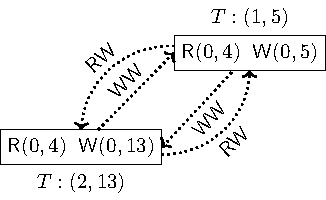
\includegraphics[width = \textwidth]{figs/galera-original}
        \caption{Original output}
    \end{subfigure}\hspace{3ex} \pause
    \begin{subfigure}[b]{0.40\textwidth}
        \centering
        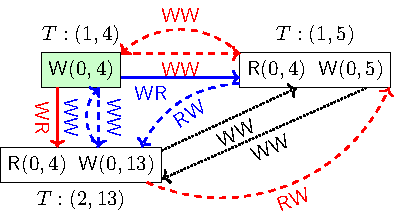
\includegraphics[width = \textwidth]{figs/galera-recovery-1}
        \caption{Missing  participants}
    \end{subfigure}\hspace{3ex} \pause
    \begin{subfigure}[b]{0.40\textwidth}
        \centering
        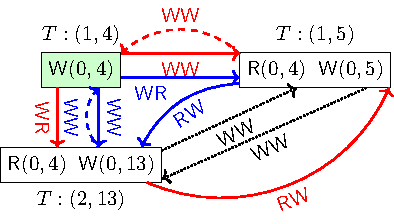
\includegraphics[width = \textwidth]{figs/galera-recovery-2}
        \caption{Recovered scenario}
    \end{subfigure}\hspace{3ex} \pause
    \begin{subfigure}[b]{0.40\textwidth}
        \centering
        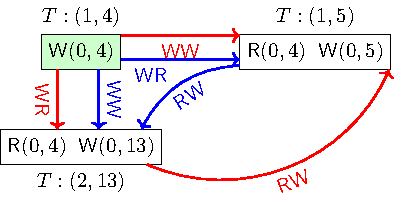
\includegraphics[width = \textwidth]{figs/galera-delete}
        \caption{Finalized scenario}
    \end{subfigure}
%     \caption{\label{ce:galera}  Lost update: the SI violation  found in MariaDB-Galera.
%     The original output dependencies  are represented by dotted black arrows.
%     The recovered dependencies are colored in red/blue with dashed and solid arrows  representing uncertain  and certain dependencies,  respectively.  The  missing transaction is colored in green.
% We omit  key 0, associated with all dependencies.    }
\end{figure}
% 	\end{center}
% \end{frame}
% %%%%%%%%%%%%%%%%%%%%

% %%%%%%%%%%%%%%%%%%%%
% \begin{frame}{Performance Evaluation}
% 	\begin{description}
% 		\setlength{\itemsep}{15pt}
% 		\item[dbcop~\ncite{Complexity:OOPSLA2019}:]
% 			the state-of-the-art SI checker
% 		\item[CobraSI:] reducing SI checking to SER checking \\
% 		  \ncite{Complexity:OOPSLA2019} to leverage Cobra with/without GPU
% 			\vspace{0.20cm}
% 			\begin{description}
% 				\item[Cobra~\ncite{Cobra:OSDI2020}:]
% 					the state-of-the-art SER checker using both MonoSAT and GPU
% 			\end{description}
% 	\end{description}
% \end{frame}
% %%%%%%%%%%%%%%%%%%%%

%%%%%%%%%%%%%%%%%%%%
\begin{frame}{}
	\centerline{\polysi{} 的性能显著优于其它 SI 检测算法。\footnote{
		本实验使用由 PostgreSQL 产生的满足 SI 的执行历史。
	}}

	\fig{width = 0.50\textwidth}{figs/polysi-runtime}
	  % {Performance comparison under various workloads ({\it timeout = $180s$}).}
  %\#sessions=20, \#txns/session=100, \#ops/txn=15,   keys=10k,  \%read=50\%, distribution=zipfian.
\end{frame}
%%%%%%%%%%%%%%%%%%%%

%%%%%%%%%%%%%%%%%%%%
\begin{frame}{}
	\centerline{\polysi{} 消耗更少的内存。}
	\fig{width = 0.50\textwidth}{figs/polysi-memory}
  %\#sessions=20, \#txns/session=100, \#ops/txn=15,   keys=10k,  \%read=50\%, distribution=zipfian.
\end{frame}
%%%%%%%%%%%%%%%%%%%%

%%%%%%%%%%%%%%%%%%%%
\begin{frame}{}
	\begin{center}
		\polysi{} 可用于检测大规模执行历史: 1M 事务, 1B 数据项

		\vspace{0.30cm}
		\fig{width = 0.70\textwidth}{figs/polysi-scalability}
		\vspace{0.30cm}
	\end{center}
\end{frame}
%%%%%%%%%%%%%%%%%%%%

%%%%%%%%%%%%%%%%%%%%
\begin{frame}{}
	\begin{center}
		\blue{剪枝 (P)} 对 \polysi{} 的性能影响较大。\footnote{
			\blue{紧凑编码 (C)} 从略。
		}

		\vspace{0.30cm}
		\fig{width = 0.70\textwidth}{figs/polysi-diff}
	\end{center}
\end{frame}
%%%%%%%%%%%%%%%%%%%%

%%%%%%%%%%%%%%%%%%%%
\begin{frame}{}
	\begin{center}
		在实验中, 剪枝步骤可以删除绝大多数约束。

		\vspace{0.30cm}
		% pruning.tex

\begin{table}[t]
	\centering
	% \caption{Number of constraints and unknown dependencies before and after  pruning (P)  in the six benchmarks.}\label{benchmark-stat}
	\renewcommand\arraystretch{1.5}
  \resizebox{0.75\textwidth}{!}{
	\begin{tabular}{c|rr|rr}
		\hline
		Benchmark  & \#cons.  & \#cons. & \#unk.  dep. & \#unk.  dep. \\
		& {before P} & \blue{\bf after P} & {before P}     & \blue{\bf after P}      \\
		\hline\hline
		TPC-C      & 386k     & \red{0}       & 3628k        & \red{0}            \\
		GeneralRH  & 4k       & 29      & 39k          & 77           \\
		RUBiS      & 14k      & 149     & 171k         & 839          \\
		C-Twitter  & 59k      & 277     & 307k         & 776          \\
		% Courseware & 156k     & 3352    & 761k         & 10359       \\
		GeneralRW  & 90k      & 2565    & 401k         & 5435         \\
		GeneralWH  & 167k     & 6962    & 468k         & 14376        \\
		\hline
	\end{tabular}}
\end{table}
		\vspace{0.30cm}

		\red{TPC-C}: 仅包含只读事务与 RMW 事务
	\end{center}
\end{frame}
%%%%%%%%%%%%%%%%%%%%
% consistency-theory.tex

%%%%%%%%%%%%%%%%%%%%%%%%%%%%%%
\begin{frame}{}
	\begin{center}
		\polysi{} 以黑盒的方式使用 MonoSAT 求解器

		\vspace{0.30cm}
		\fig{width = 0.70\textwidth}{figs/solver-blackbox}
		\vspace{0.30cm}

		未能充分利用 SAT/SMT 搜索框架 (DPLL/CDCL)
	\end{center}
\end{frame}
%%%%%%%%%%%%%%%%%%%%%%%%%%%%%%

%%%%%%%%%%%%%%%%%%%%%%%%%%%%%%
\begin{frame}{}
	\begin{center}
		\blue{\bf 当前的探索:} 如何``深度整合 SMT'', 进一步提升算法效率?

		\vspace{0.50cm}
		\fig{width = 0.70\textwidth}{figs/integrated}
	\end{center}
\end{frame}
%%%%%%%%%%%%%%%%%%%%%%%%%%%%%%

%%%%%%%%%%%%%%%%%%%%%%%%%%%%%%
\begin{frame}{}
	\begin{center}
		多线程程序验证问题~\ncite{Zord:PLDI2021}

		\vspace{0.30cm}
		\fig{width = 0.90\textwidth}{figs/pldi2021}
	\end{center}
\end{frame}
%%%%%%%%%%%%%%%%%%%%%%%%%%%%%%

%%%%%%%%%%%%%%%%%%%%%%%%%%%%%%
\begin{frame}{}
	\begin{center}
		设计专用的事务一致性理论求解器 (图片来自~\ncite{Zord:PLDI2021})

		\vspace{0.50cm}
		\fig{width = 0.65\textwidth}{figs/smt-framework}
	\end{center}
\end{frame}
%%%%%%%%%%%%%%%%%%%%%%%%%%%%%%

%%%%%%%%%%%%%%%%%%%%%%%%%%%%%%
\begin{frame}{}
	\fig{width = 0.95\textwidth}{figs/consistency-theory-solver-revised}

	%	\begin{itemize}
	%		\item \textcolor[RGB]{71,46,125}{\textbf{Pick}}: select a variable to make an assignment
	%		\item \textcolor[RGB]{71,46,125}{\textbf{T}}heory\textcolor[RGB]{71,46,125}{\textbf{-Propagate}}: efficiently detect possible cycle upon inserting arcs
	%		\item \textcolor[RGB]{71,46,125}{\textbf{T}}heory\textcolor[RGB]{71,46,125}{\textbf{-Analyze}}: find proper cycle(s)
	%		\item \textcolor[RGB]{71,46,125}{\textbf{Unit-edge Propagate}}: derive literatures from current reachability
	%	\end{itemize}
\end{frame}
%%%%%%%%%%%%%%%%%%%%%%%%%%%%%%

%%%%%%%%%%%%%%%%%%%%%%%%%%%%%%
\begin{frame}{}
	\begin{center}
		增量式环检测算法~\ncite{ICD:TOA2015} 与 Unit-edge Propagation

		\vspace{0.50cm}
		\fig{width = 0.95\textwidth}{figs/ICD-algorithm-and-unit-edge-propagation.png}
	\end{center}

	% takes at most $O(\min\{m^{1/2}, n^{2/3}\}m)$ time to insert $m$ arcs into an $n$-vertex graph.
\end{frame}
%%%%%%%%%%%%%%%%%%%%%%%%%%%%%%

%%%%%%%%%%%%%%%%%%%%%%%%%%%%%%
\begin{frame}{}{pruning, pair conflict generation, ...}
	\begin{center}
		剪枝: ``小环''占多数, 可以用于排除不可能的约束
	\end{center}

	\begin{figure}[H]
		\centering
		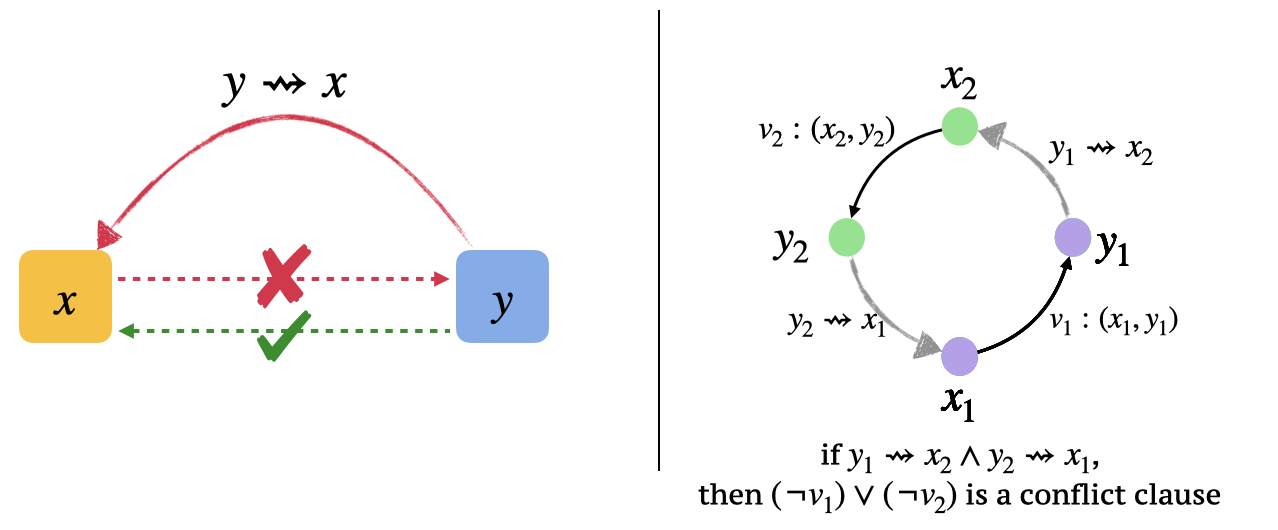
\includegraphics[width=0.9\textwidth]{figs/pruning-and-pair-conflict-generation.png}
	\end{figure}
\end{frame}
%%%%%%%%%%%%%%%%%%%%%%%%%%%%%%

%%%%%%%%%%%%%%%%%%%%%%%%%%%%%%
% \begin{frame}{}
% 	% \begin{center}
% 	% 	\scriptsize{
% 	% 		\begin{tabular}{|c|c|c|c|c|}
% 	% 			\hline
% 	% 			baseline & \makecell{cycle\\ detection} & \makecell{conflict\\ generation} & \makecell{unit-edge\\ propagation} & \makecell{pair conflict\\generation} \\
% 	% 			\hline
% 	% 			z3 user propagator* & local toposort & smallest & $\checkmark$(partial) & \\
% 	% 			\hline
% 	% 			monosat & PK toposort & first & & \\
% 	% 			\hline
% 	% 			acyclic minisat* & ICD & first & $\checkmark$ & $\checkmark$ \\
% 	% 			\hline
% 	% 			cobra(w/o GPU) & \multicolumn{3}{c|}{same as monosat} & \\
% 	% 			\hline
% 	% 		\end{tabular}
% 	% 	}
% 	% 	\\
% 	% 	\tiny{*: we implemented}
% 	% \end{center}

% 	\begin{figure}[H]
% 		\centering
% 		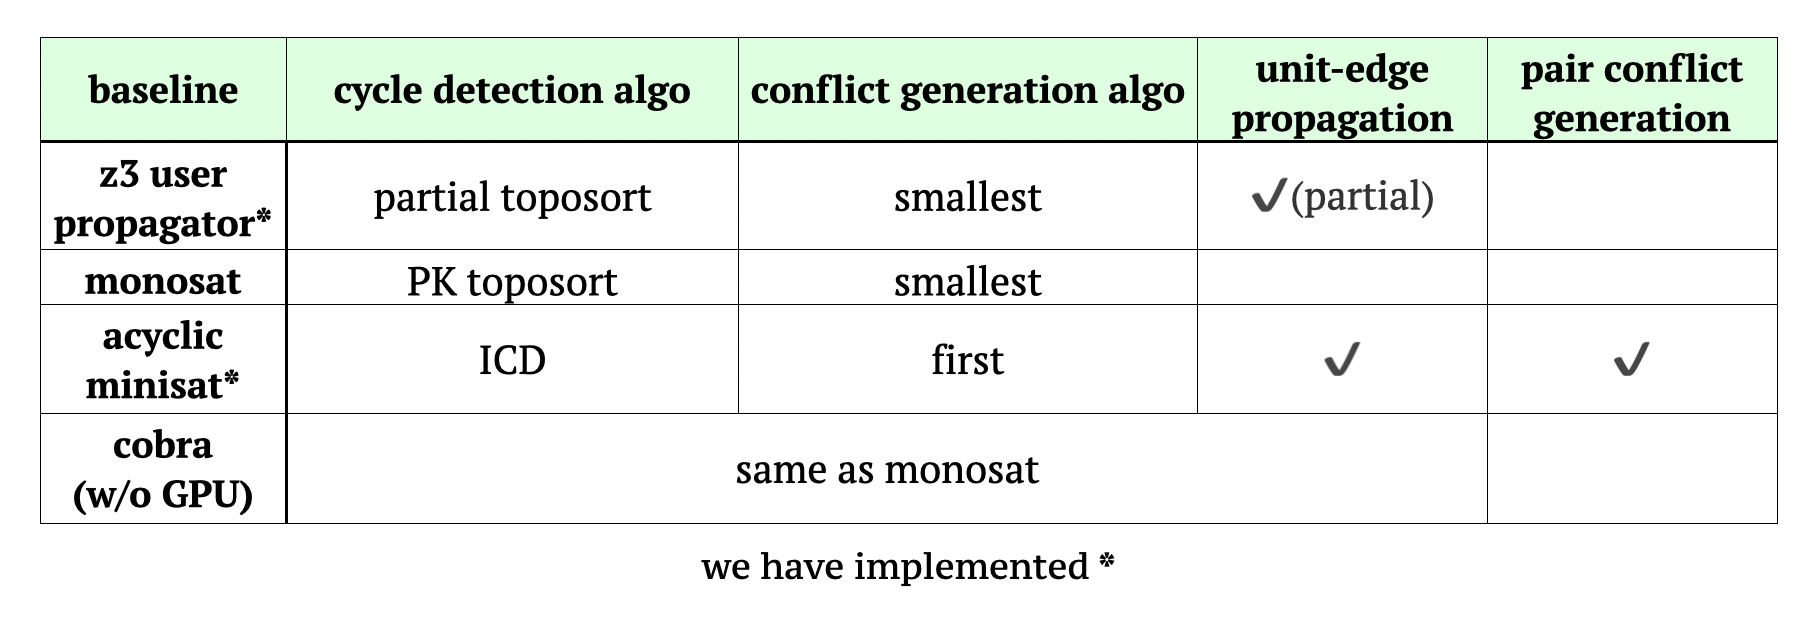
\includegraphics[width=\textwidth]{figs/ser-checker-baselines.png}
% 	\end{figure}
% \end{frame}
%%%%%%%%%%%%%%%%%%%%%%%%%%%%%%

%%%%%%%%%%%%%%%%%%%%%%%%%%%%%%
\begin{frame}{}
	\begin{center}
		``可序列化''一致性模型检测算法性能对比\blue{\bf 初步结果}
	\end{center}

	\begin{figure}[H]
		\centering
		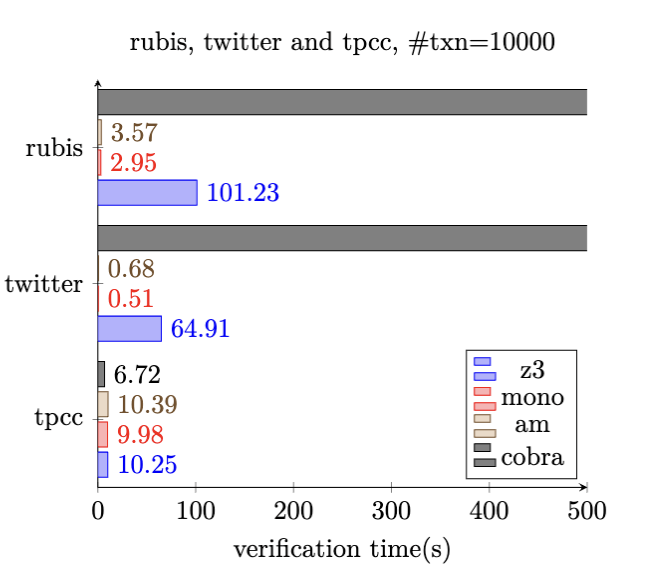
\includegraphics[width=0.48\textwidth]{figs/ser-checker-rubis-twitter-and-tpcc-ntxn10000.png}
		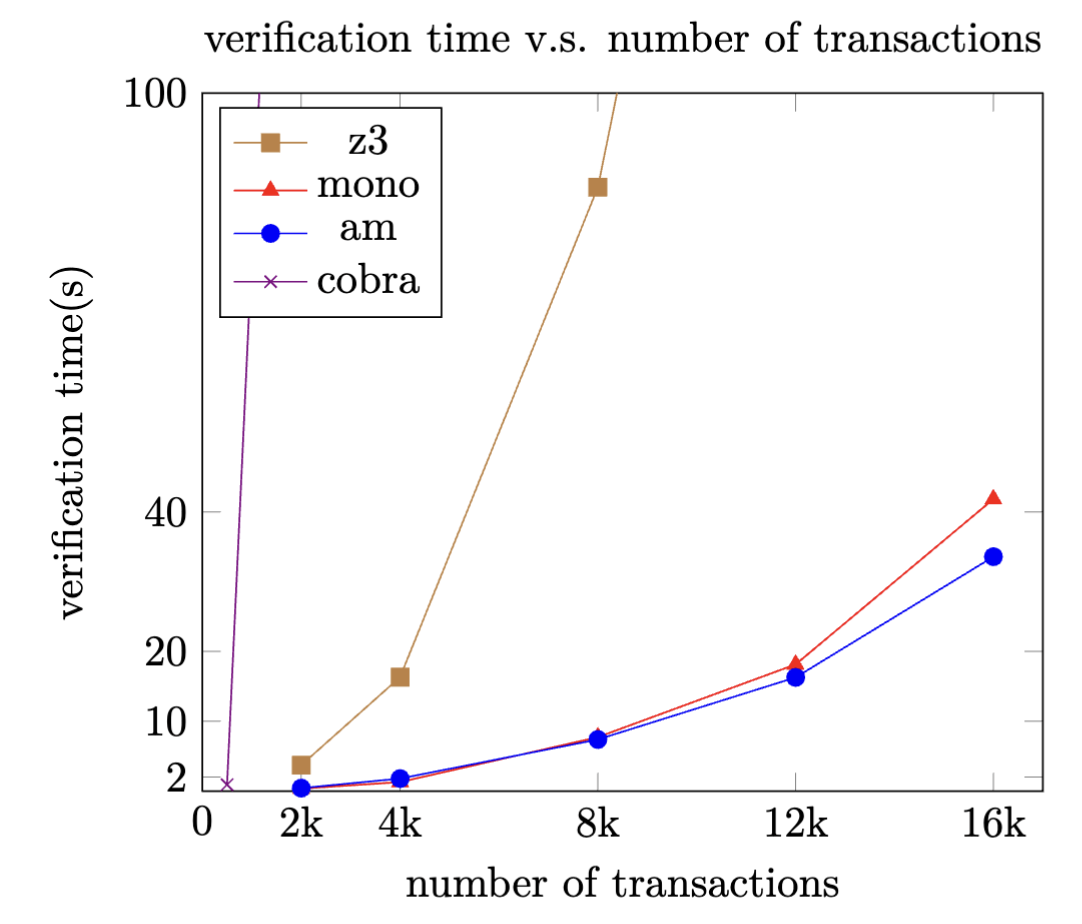
\includegraphics[width=0.48\textwidth]{figs/ser-checker-chengRW-verification-time-vs-ntxns.png}
	\end{figure}
\end{frame}
%%%%%%%%%%%%%%%%%%%%%%%%%%%%%%

% %%%%%%%%%%%%%%%%%%%%%%%%%%%%%%
% \begin{frame}{What Needs To Do Next}
% 	\begin{itemize}
% 		\item \textbf{pick}: leverage the underlying graph infomation to make a seemingly best assignment.
% 		\begin{itemize}
% 			\item to choose the variable that contains maximum / minimal edges, or is able to best trigger unit-edge propagation.
% 			\item to learn some infomation from those detected cycles.
% 		\end{itemize}
% 		\item \textbf{unify the approach to handle small width cycles}
% 		\begin{itemize}
% 			\item to design an algorithm that performs well on those small width cycles.
% 		\end{itemize}
% 		\item \textbf{make the theory solver lazier}
% 		\begin{itemize}
% 			\item observation: after pruning and pair conflict generation, the times of detecting a cycle has declined greatly.
% 			\item a lazier theory solver may be capable for big yet powerful cycle detection algorithms.
% 		\end{itemize}
% 	\end{itemize}
% \end{frame}
% %%%%%%%%%%%%%%%%%%%%%%%%%%%%%%
% conclusion.tex

%%%%%%%%%%%%%%%%%%%%
\begin{frame}{}
	\begin{center}
		\fig{width = 0.90\textwidth}{figs/roadmap}
	\end{center}
\end{frame}
%%%%%%%%%%%%%%%%%%%%
%%%%%%%%%%%%%%%%%%%%
\thankyou{}
%%%%%%%%%%%%%%%%%%%%
% cite references using \ncite{} and compile with biber
% \begin{frame}[allowframebreaks]
%   \printbibliography
% \end{frame}
%%%%%%%%%%%%%%%%%%%%
% \appendix

\end{document}
%%%%%%%%%%%%%%%%%%%%